%%%%%%%%%%%%%%%%%%%%%%%%
% 2) Setting CMake Options (Public)
%%%%%%%%%%%%%%%%%%%%%%%%

The CMake program is used to set additional options for the \ac{EMTG} build.

\begin{enumerate}
	\item Open the CMake \ac{GUI}.
	\item Make sure that the ``Advanced'' and ``Grouped'' check boxes are checked. \\ \emph{This makes it easier to see all options.}
	\item In the ``Where to build the binaries:'' text box, put \textbf{\textless EMTG\_root\_dir\textgreater}/build. \\ \emph{It is OK if the ``build'' directory does not exist yet; CMake will create it.}
	\item In the ``Where is the source code:'' text box, put \textbf{\textless EMTG\_root\_dir\textgreater}.
	\item Click ``Configure'' button.
	\item Select the options you want for each ``Name'' in the ``Value'' column. 
	\begin{enumerate}
		\item Select and confirm the appropriate SNOPT settings by following the steps below:
		\begin{enumerate}
			\item Expand the ‘Ungrouped Entries’ section
			\item Ensure SNOPT\_MINGW\_DLL is checked 
				\begin{figure}[H]
					\centering
					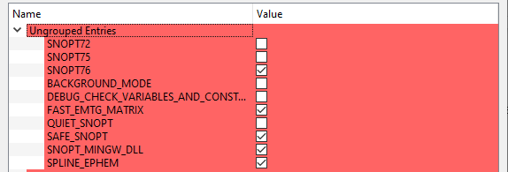
\includegraphics[width=0.7\linewidth]{../../../shared_latex_inputs/images/emtg_cmake_ungrouped-options.png}
					\caption{EMTG CMAKE Ungrouped Entries Selection}
				\end{figure}
		\end{enumerate}
		\item Ensure all the options under ``HAS'' are checked: \\ \emph{Note that for the current public release these options are not fully functional}
		\begin{enumerate}
			\item Expand the ``HAS'' section
			\item Check the HAS\_BUILT\_IN\_THRUSTERS option
			\item Check the HAS\_PROBEENTRYPHASE option 
				\begin{figure}[H]
					\centering
					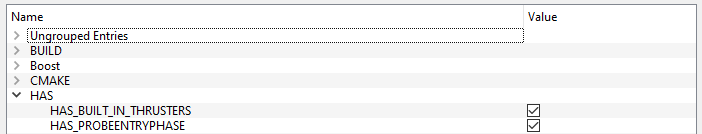
\includegraphics[width=0.75\linewidth]{../../../shared_latex_inputs/images/emtg_cmake_has-options.png}
					\caption{EMTG CMAKE Has Selection}
				\end{figure}
		\end{enumerate}
		\item Ensure Boost was detected by following the steps below:
		\begin{enumerate}
			\item Expand the ``Boost'' section
			\item Verify the directories have autopopulated to the correct location in which Boost is installed
		\end{enumerate}
		\item Enable the pyhardware and propulator utility by following the steps below:
		\begin{enumerate}
			\item Expand the ``BUILD'' section 
			\item Check the ``BUILD PROPULATOR'' option
			\item Check the ``BUILD PYHARDWARE'' option
		\end{enumerate}
	\end{enumerate}
	\item Click ``Configure''
	\item Configure the Python settings to point to the appropriate PyEMTGEnv paths:
		\begin{enumerate}
			\item Expand the ``PYTHON'' section
				\begin{enumerate}
					\item Sometimes the ``PYTHON'' section is not populated when Python is not found. You may need to update the ''Ungrouped Entries'' and populate the PYTHON\_EXECUTABLE as indicated in the next step then click ``Configure'' to see the other parameters mentioned in the next step.
				\end{enumerate}
			\item Replace the Python paths in the PYTHON\_EXECUTABLE, PYTHON\_INCLUDE\_DIR, and PYTHON\_LIBRARY values to point to where your PyEMTGEnv is located (e.g. \verb|C:/Users/YourName/AppData/Local/mambaforge/envs/PyEmtgEnv/*|)
		\end{enumerate}
	\item Click ``Configure''
	\item Click ``Generate''
	\item Click the ``Open Project'' button \\ \emph{This will launch the Visual Studio application}
\end{enumerate}